\documentclass[a4paper,12pt,notitlepage]{report}

% Packages
\usepackage[utf8]{inputenc}
\usepackage[T1]{fontenc} 
\usepackage[francais,english]{babel}
\usepackage{graphicx}
\usepackage{biblatex}
\usepackage[export]{adjustbox}

% Counters for toc and numerotation depth
%\setcounter{tocdepth}{1}
\setcounter{secnumdepth}{1}

\graphicspath{{images/}}

\begin{document}

\begin{titlepage}
	\centering
	
\includegraphics[width=0.6\textwidth]{hearc_logo}\par
	\vspace{1cm}
	{\scshape\Large \par}
	\vspace{1.5cm}
	{\huge\bfseries ARC3D\par}
	\vspace{0.5cm}
	{\small Travail de Bachelor - 16dlm-tb-219\par}
	\vspace{2cm}
	{\Large Thomas \bsc{Roulin}\par}
	\vfill
	encadrement pédagogique par\par
	Stéphane \textsc{Gobron}
	
	\vfill
	
	% Bottom of the page
	{\large \today\par}
\end{titlepage}

% Abstract in both languages
\vspace*{\fill}
\selectlanguage{francais}
\begin{abstract}
	
	Le Campus Arc 2 de la Haute-École Arc, (HE-Arc), Neuchâtel, HES-SO, est un bâtiment de grande envergure dont certaines zones ont dû être sécurisées. Des open-spaces, dont l'accès est réglementé et limité, engendrent des problèmes tant pour les visiteurs que pour les étudiants. Il est régulièrement difficile de savoir, selon le type d'utilisateur, quel chemin emprunter. Un outil facilitant les déplacements, en permettant la visualisation et le tracé du chemin pour se rendre en tout lieu et en toute salle du campus, pourrait résoudre ce problème. Ce rapport décrit le développement dudit outil, lequel facilite les déplacements à l'intérieur du bâtiment mais englobe également les déplacements depuis la gare au campus. %En résumé, le point de départ peut tout aussi être un endroit dans le bâtiment qu'un autre se trouvant dans la gare de Neuchâtel.
	
	La solution apportée se présente sous la forme d'une page Internet accessible depuis un smartphone ou un ordinateur. La technologie utilisée est celle du WebGL, ce qui évite tous les problèmes de librairies externes ou de plugins.
	
\end{abstract}

\selectlanguage{english} 
\begin{abstract}
	Karim halp me pls.
\end{abstract}
\vspace*{\fill}
\selectlanguage{francais}

% ToC
\tableofcontents

% Content
\chapter{Introduction}

\section{Problématique générale}
Au XXIe siècle, tout va toujours plus vite, l'être humain n'entend pas perdre de temps inutilement et, notamment, pas pour chercher son chemin. Pour se déplacer sur un site d'une certaine complexité et d'une certaine envergure, il convient d'offrir une aide au déplacement, sous la forme d'une solution rapide et facile d'accès. L'utilisation de la 3D en navigateur n'est que très peu répandue pour l'instant, mais elle pourrait tout à fait répondre à ce besoin. Proposer un tel outil, innovant et performant, aurait également l'avantage de répondre à une certaine ambition du domaine Ingénierie de l'HE-Arc de Neuchâtel, en matière de visualisation en temps réel.   


\section{Contextualisation}
Dans le cadre du Campus Arc 2, le deuxième étage est considéré comme un open space. La particularité est que différents secteurs sont fermés aux visiteurs et élèves. Outre sa dimension, c'est une des causes principales de problèmes de déplacements à l'intérieur du bâtiment. Il est ainsi fondamentalement intéressant d'offrir un outil pour faciliter les trajets à l'intérieur du bâtiment et depuis la gare.


\chapter{Analyse}
Présentation du problème, les solutions. Comment il a été découpé.
Concepts et justifications.
\section{État de l'art}
Avant de démarrer le développement il est important de se renseigner sur les travaux qui ont déjà été effectués concernant des objectifs du projet.
\subsection{3D temps réel}
\subsection{Navigation}
\subsection{Architecture}
\section{Localisation en intérieur}
Un challenge principal était la localisation en intérieur de l'utilisateur. C'est intéressant pour l'utilisateur s'il a un suivi régulier de sa position durant la visualisation 3D. Cette section va expliquer les diverses pistes empruntées ainsi que leurs résultats.

\subsection{GPS}
Quand on entend localisation on pense très vite au GPS (\textit{Global Positioning System}) qui pourrait présenter une bonne solution à première vue. Cependant cette technologie manque de précision, principalement en intérieur. La précision des GPS mobiles se situerait à peu près entre 4 et 50 mètres, dépendant des conditions et du smartphone utilisé. En général, l'erreur est due aux éléments entre l'utilisateur et le satellite, c'est pourquoi la localisation en intérieur ne peut pas se fier au GPS.

\subsection{Triangulation Wifi}
Une méthode utilisé pour la localisation en intérieur est la triangulation / trilateration en utilisant les \textit{Access Points} WiFi. Le concept est d'avoir à l'avance retenu les coordonnées de tous les AP. Chaque AP possède une adresse MAC qui les différencie les uns des autres. Ensuite il faut scanner les AP depuis l'objet que l'ont veut localiser et en fonction des forces des AP il est possible de retrouver sa position.

L'avantage de cette solution est qu'il n'y a pas d'infrastructure à mettre en place, étant donné que le Campus est déjà équipé de bon nombre d'AP. Cependant le but de ce projet est d'offrir une application dans un navigateur Internet. Cette contrainte nous empêche d'accéder à n'importe quelle information de l'appareil qui l'utilise. Malgré les technologies qu'offre ce monde il est encore impossible de récupérer les informations nécessaires à la triangulation / trilatération depuis une page web.

\subsection{Triangulation Bluetooth}
Une autre manière d'utiliser la triangulation est de mettre en place des beacons bluetooth. Il s'agit de petits émetteurs que l'on place dans l'espace où l'on veut localiser l'utilisateur. Le fonctionnement de la triangulation est pareil que pour le WiFi.


Sans compter le désavantage qu'est la mise en place de l'infrastructure, les accès bluetooth depuis une page web ne sont pas encore assez supportés. Le tableau \ref{caniuse-bluetooth} tiré du site www.caniuse.com montre que seul Chrome le supporte ssi on active le drapeau nécessaire. Ceci démontre que l'API Web Bluetooth n'est pas utilisable pour une application destinée au grand public.

\begin{figure}[h!]
	\center
	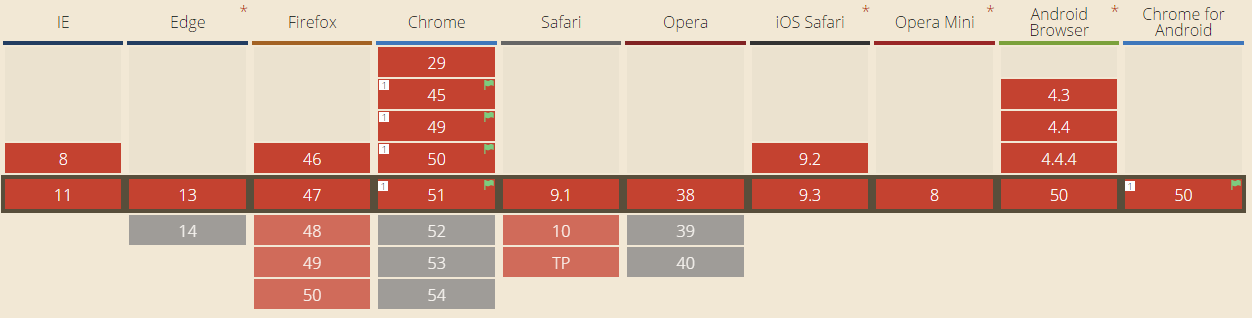
\includegraphics[width=10cm,frame]{caniuse_bluetooth}
	\caption{Support de l'API Web Bluetooth par les différents navigateurs.}
	\label{caniuse-bluetooth}
\end{figure}

\subsection{Accéléromètre et Gyroscope}
L'approche ici est différente, nous désirons utiliser les capteurs internes du smartphone afin de calculer une position. HTML5 fournit une API pour détecter l'orientation et les déplacements du dispositif. Autrement dit, nous avons accès à l'accéléromètre et au gyroscope depuis un navigateur Internet.

A l'aide de l'accélération il est théoriquement possible de calculer une position. Cependant les valeurs de ces capteurs comportent un bruit et pour calculer une position il faut double-intégrer l'accélération. Cela signifie que nous devrons double-intégrer le bruit et cela va créer un \textit{drift}, en quelques secondes l'erreur peut s'élever à une vingtaine de centimètres. En outre, le gyroscope peut avoir une valeur erronée due à la suppression de la gravité. C'est-à-dire que si nous avons une erreur d'un degré sur la valeur du gyroscope, en quelques seconde l'erreur s'élève à plusieurs mètres cette fois. Citer https://youtu.be/C7JQ7Rpwn2k?t=23m22s

Le but de cette approche était d'estimer la position de l'utilisateur sans pour autant connaître la valeur exacte. Les résultats prouvent que même une approximation n'est pas envisageable avec ces capteurs.

\chapter{Développement}
\section{Modèle}
Explication des différents problèmes rencontrés avec le modèle, son texturing, son exportation et importation.

\subsection{Modélisation}
Citer Kevin ?
Seulement les plans de sols et pas de coupe. Approximation par ratio des hauteurs.

\subsection{Texturisation}
Application des textures.
Erreur export de fichier, modification du script d'exportation.

\subsection{Import/Export}
Type d'objet utilisé.`Contraintes/avantages.
\section{Rendu graphique}
Matériaux de Lambert
Éclairage.

\section{Recherche de chemin}

\subsection{Nœuds}
Format
Placement dans l'espace

\subsection{Algorithme}
A-Star
\section{Contrôles de la caméra}
L'application a pour but d'être utilisée sur mobile et tablette mais cela n'empêche pas qu'elle soit accessible par un ordinateur. Cela implique qu'il faudra gérer de manière différente ces deux types de clients. Afin de détecter à quel type d'appareil la page doit répondre, la meilleure technique est encore d'utiliser une expression régulière sur le \emph{User agent} \cite{wiki-useragent}.

\subsection{Orientation mobile}
Sur un ordinateur, il est possible de se déplacer à l'aide des touches fléchées. Sur un mobile, on ne peut pas utiliser le même fonctionnement. L'idée est d'utiliser le gyroscope interne du smartphone à l'aide de l'API \emph{DeviceOrientation \& DeviceMotion events}\cite{w3c-orientation} supporté par tous les navigateurs mobiles\cite{caniuse-DeviceMotion}. 

Le senseur nous envoie alpha, beta et gamma qui sont respectivement les rotations sur les axes Z, X' et Y'', voir Figure \ref{fig:mobile-angles}. On peut en déduire facilement les angles d'\emph{Euler}, puis il est possible d'en trouver le quaternion qui exprime la rotation que l'on applique ensuite à notre caméra. Cependant, les smartphones n'envoient pas forcément des valeurs absolues, c'est-à-dire qu'il n'est pas possible de trouver le nord à partir de ces valeurs. Le magnétomètre n'est pas accessible depuis une page web, ce qui aurait pu nous aider à trouver le nord. L'interface utilisateur permet de décaler la valeur alpha du gyroscope à gauche ou à droite, afin de pouvoir calibrer à la main son orientation.

\begin{figure}
	\centering
	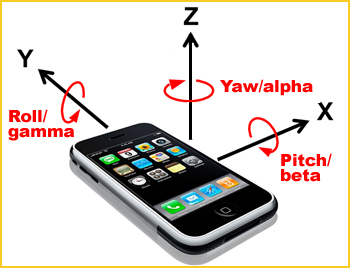
\includegraphics[width=0.4\linewidth]{mobile-sensors}
	\caption{Les axes ainsi que leurs rotations respectives du téléphone mobile. Source image: \url{http://hillcrestlabs.com}}
	\label{fig:mobile-angles}
\end{figure}

\subsection{Suivi du chemin}
Après que l'utilisateur ait choisi un point A et un point B, l'algorithme de recherche de chemin va définir un itinéraire à suivre. La caméra doit parcourir ce chemin, tout en gardant une certaine orientation afin que l'utilisateur puisse le comprendre. Afin que les contours soient plus naturels et moins brutaux, il est important d'interpoler les points que l'on doit suivre. Dans le cas d'Arc3D, c'est une interpolation avec méthode de Catmull-Rom qui est utilisée. Ceci pour la raison que cette méthode fonctionne avec autant de points que nécessaires et qu'il s'agit d'une méthode déjà connue de ma part.

Il reste encore un problème : si le mode \textit{à mobilité réduite} est activé, la recherche de chemin va plutôt emprunter les ascenseurs que les escaliers. Dans ce cas-là, on va créer des courbes supplémentaires, pour chaque section du tracé, voir figure \ref{fig:spline-stairselevator}. Le programme calcule la distance parcourue de l'utilisateur et détermine sur laquelle des courbes il se trouve.

\begin{figure}
	\centering
	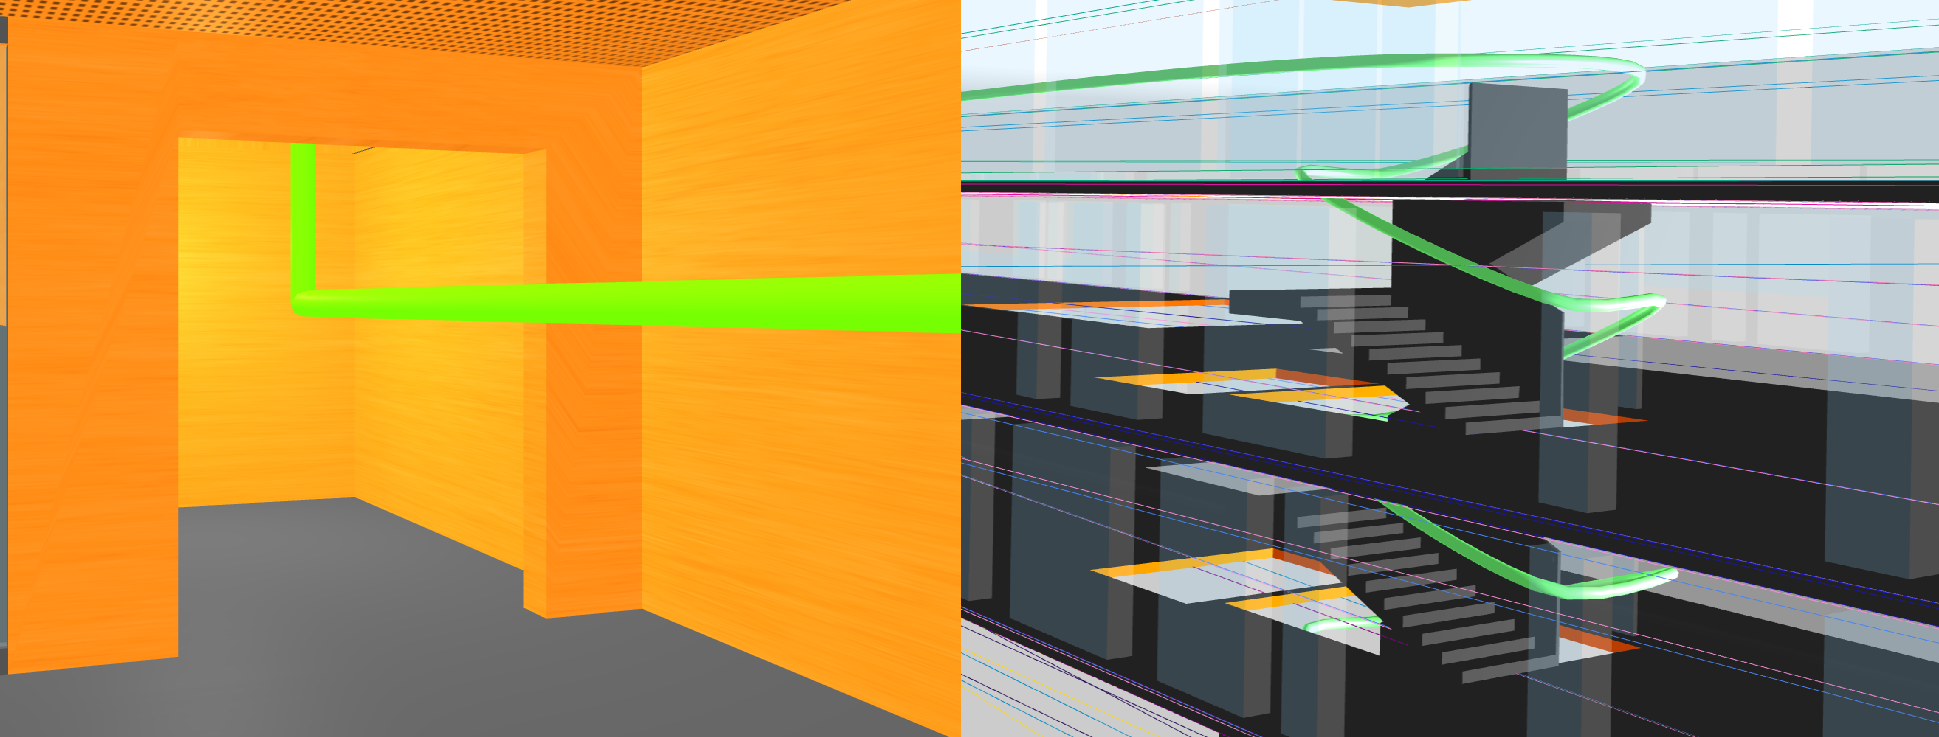
\includegraphics[width=0.9\linewidth]{spline-StairsElevator}
	\caption{La différence entre une courbe qui passe par les escaliers ou un ascenseur.}
	\label{fig:spline-stairselevator}
\end{figure}

Ensuite, il reste à définir la direction de la caméra. Comme expliqué avant, il y a une courbe pour chaque section du tracé. Chacune d'elles est liée à un comportement qui est différent pour les ascenseurs (\textit{elevator behaviour}) et pour les autres sections (\textit{normal behaviour}). Le comportement de type \emph{normal} va simplement regarder un point qui se trouve à une certaine distance devant l'utilisateur sur la courbe. Tandis que le comportement \emph{elevator} est décrit comme suit: 
au début d'une courbe \emph{elevator}, on stocke un vecteur unitaire dans la dernière direction de la courbe précédente et un deuxième dans la première direction de la courbe suivante. Ensuite, tout au long du trajet, on effectue une interpolation linéaire entre les deux vecteurs directeurs calculés précédemment. Cela permet d'imiter le comportement d'un humain dans un ascenseur, comportement qui l'amène généralement à pivoter sur lui-même pour être prêt à sortir du bon côté de l'ascenseur.

\subsubsection{Live et Simulation}
L'application propose encore deux modes de visualisation différents, lesquels ont été nommés \emph{Live} et \emph{Simulation}. Le mode \emph{Live} devait à la base représenter le mode dans lequel l'utilisateur était géolocalisé en permanence. Étant donné que cet objectif n'est pas réalisable, c'est un autre mécanisme qui a été mis en place. La visualisation procède au déplacement seulement si l'orientation du téléphone regarde dans la direction du chemin. Tandis que le mode \emph{Simulation} se déplace continuellement et que la caméra est fixée sur le chemin.

\section{Suivi caméra}
Les méthodes que nous avons décidé d'implémenter, à savoir \textit{Live Mode} et \textit{Simulation mode}.

\subsection{Lissage du chemin}
Catmull Rom

\subsection{Regard de la caméra}
Comment la caméra sait où regarder.
\section{Interface graphique}
Toucher un mot sur l'interface graphique.

\section{Rendu temps réel}
je l'ai testé sur 3 trucs. minimum 30 fps

\chapter{Résultats}
Lister les objectifs, lesquels sont réussi, pourquoi les autres le sont pas...
\section{Temps réel}
\section{Modélisation géométrique}
\section{Réalisation des objectifs}

\chapter{Discussion}
\section{Conclusion}
\section{Perspectives}
Objectifs pas réussis : Comment les réussir.

Améliorations possibles.

Pas de perspectives faciles.


\chapter{Bibliographie}

\end{document}